%%%%%%%%%%%%%%%%%%%%%%%%%%%%%%%%%%%%%%%%%
% Beamer Presentation
% LaTeX Template
% Version 1.0 (10/11/12)
%
% This template has been downloaded from:
% http://www.LaTeXTemplates.com
%
% License:
% CC BY-NC-SA 3.0 (http://creativecommons.org/licenses/by-nc-sa/3.0/)
%
%%%%%%%%%%%%%%%%%%%%%%%%%%%%%%%%%%%%%%%%%

%----------------------------------------------------------------------------------------
%	PACKAGES AND THEMES
%----------------------------------------------------------------------------------------

\documentclass{beamer}

\usepackage[utf8]{inputenc}
\usepackage[english,russian]{babel}

\mode<presentation> {

% The Beamer class comes with a number of default slide themes
% which change the colors and layouts of slides. Below this is a list
% of all the themes, uncomment each in turn to see what they look like.

%\usetheme{default}
%\usetheme{AnnArbor}
%\usetheme{Antibes}
%\usetheme{Bergen}
%\usetheme{Berkeley}
%\usetheme{Berlin}
%\usetheme{Boadilla}
%\usetheme{CambridgeUS}
%\usetheme{Copenhagen}
%\usetheme{Darmstadt}
%\usetheme{Dresden}
%\usetheme{Frankfurt}
%\usetheme{Goettingen}
%\usetheme{Hannover}
%\usetheme{Ilmenau}
%\usetheme{JuanLesPins}
%\usetheme{Luebeck}
\usetheme{Madrid}
%\usetheme{Malmoe}
%\usetheme{Marburg}
%\usetheme{Montpellier}
%\usetheme{PaloAlto}
%\usetheme{Pittsburgh}
%\usetheme{Rochester}
%\usetheme{Singapore}
%\usetheme{Szeged}
%\usetheme{Warsaw}

% As well as themes, the Beamer class has a number of color themes
% for any slide theme. Uncomment each of these in turn to see how it
% changes the colors of your current slide theme.

%\usecolortheme{albatross}
%\usecolortheme{beaver}
%\usecolortheme{beetle}
%\usecolortheme{crane}
%\usecolortheme{dolphin}
%\usecolortheme{dove}
%\usecolortheme{fly}
%\usecolortheme{lily}
%\usecolortheme{orchid}
%\usecolortheme{rose}
%\usecolortheme{seagull}
%\usecolortheme{seahorse}
%\usecolortheme{whale}
%\usecolortheme{wolverine}

%\setbeamertemplate{footline} % To remove the footer line in all slides uncomment this line
%\setbeamertemplate{footline}[page number] % To replace the footer line in all slides with a simple slide count uncomment this line

%\setbeamertemplate{navigation symbols}{} % To remove the navigation symbols from the bottom of all slides uncomment this line
}

\usepackage{graphicx} % Allows including images
\usepackage{booktabs} % Allows the use of \toprule, \midrule and \bottomrule in tables

%для ссылок
\usepackage{xcolor}
\usepackage{hyperref}
\definecolor{linkcolor}{HTML}{799B03} % цвет ссылок
%\definecolor{urlcolor}{HTML}{799B03} % цвет гиперссылок
\hypersetup{pdfstartview=FitH,  linkcolor=linkcolor, urlcolor=blue
	, colorlinks=true}

%----------------------------------------------------------------------------------------
%	TITLE PAGE
%----------------------------------------------------------------------------------------

%\title[Short title]{Full Title of the Talk} % The short title appears at the bottom of every slide, the full title is only on the title page
%
%\author{John Smith} % Your name
%\institute[UCLA] % Your institution as it will appear on the bottom of every slide, may be shorthand to save space
%{
%University of California \\ % Your institution for the title page
%\medskip
%\textit{john@smith.com} % Your email address
%}
%\date{\today} % Date, can be changed to a custom date

\begin{document}

\section{Basics}


\begin{frame}
\frametitle{Notation}
$L(y, \hat y)$ -- loss function differentiable by $\hat y$. \par
$X, y = \{x_1, \ldots ,x_N\}, \{y_1, \ldots ,y_N \}$ -- data. \par
$\mathcal{H}$ -- class of base learners (aka weak learners). \par
We will suppose that $\mathcal{H}$ is closed under multiplication by constants. \par
We want to build model as a sum of $T$ base learners:
$$F(x) = \sum_{i = 0}^{T - 1} f_i(x), \quad f_i \in \mathcal{H}$$
We greedily minimize an empirical loss $L(F) = \sum_{i=1}^N L(y_i, F(x_i))$

\end{frame}

\begin{frame}
\frametitle{Notation}
$F_t(x) = \sum_{i = 1}^{t-1} f_i(x)$ -- our model at iteration t. Let:\par
$$g_i = -\frac{\partial}{\partial \hat y} L(y_i, \hat y)|_{\hat y = F_t(x_i)} \quad \mbox{(antigradients)}$$
$g_i$ is a vector if $\hat y$ is a vector.\par
And hopefully we will succeed to talk about second derivatives:
$$h_i = \frac{\partial^2}{\partial^2 \hat y} L(y_i, \hat y)|_{\hat y = F_t(x_i)}$$
We assume $h_i$ to be positive (i.e. that $L$ is convex in $\hat y$).

\end{frame}

\begin{frame}
\frametitle{Vanilla gradient boosting}
Let's add base learner $f$ to $F_t$.\par
Let $g = (g_1, \ldots, g_N)$ and $f(X) = (f(x_1), \ldots, f(X_N))$ \par
Because $f$ is supposed to be small we can use first order loss approximation:
$$ L(F_t + f) = \sum_{i=1}^N L(y, F_t(x_i) + f(x_i)) = L(F_t) -\langle g, f(X)\rangle + o(\|f(X)\|) = $$
$$ L(F_t) - \cos(g, f(X)) \cdot \|g\| \cdot \|f(X)\| + o(\|f(X)\|)$$
So steepest descent achieves $f$ which maximize $\cos(g, f(X))$ \par
Or minimize $\|g - f(X) \|^2 \geqslant |\sin(g, f(X)) \cdot \|g\||^2$

\end{frame}

\begin{frame}
\frametitle{Geometric proof}

$$argmax_{f\in \mathcal{H}} \cos(g, f(X)) = argmin_{f\in \mathcal{H}} \|g - f(X) \|^2 $$
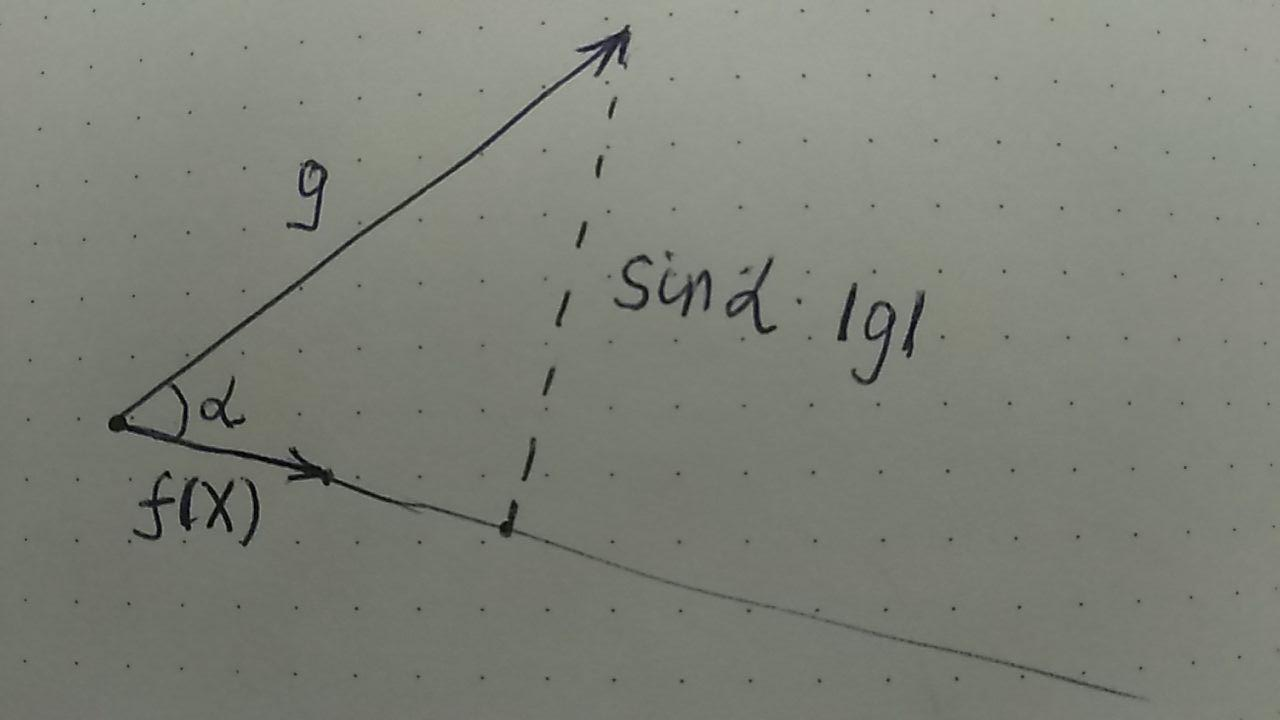
\includegraphics[width=120mm]{cos_mse_equivalence.jpg}
%\caption{}
%\label{}

\end{frame}

\begin{frame}[fragile]
\frametitle{Pseudocode}
\href{https://en.wikipedia.org/wiki/Gradient_boosting#Algorithm}{see pseudocode here} \par
What to tell:
\begin{itemize}
	\item Learning rate. It's called shrinkage sometimes (like one other thing).
	\item Line search (from wiki pseudocode) sucks.
	\item Gradient boosting is an inferior approximation of simple boosting.
	\item Greedy trees.
	\item Other score functions (like 'mae' in sklearn) are strange.
\end{itemize}
\end{frame}

\section{Tree scoring}

\begin{frame}
\frametitle{More notation}
Tree consists of its structure and leaf values. \par
Suppose we have some fixed tree structure. Then \par
\begin{itemize}
	\item $V$ -- space of leaf values.
	\item $T_{\hat y} \approx \mathbb{R}^N$ -- space of predictions.
	\item $A: V \to T_{\hat y}$ linear mapping defined by tree structure ($A_{ij} \in\{0, 1\}$ indicates if object $i$ hits leaf $j$).
	\item $W$ -- matrix of scalar product on $T_{\hat y}$ (np.diag(object\_weights)).
\end{itemize}
\end{frame}

\begin{frame}
\frametitle{Suddenly, main optimization formula}
Let $g \in \mathbb{R}^n$, $A$ -- simmetric, positively definite.
$$ \mathrm{argmin}_{v} \left(-\langle g, v\rangle + \frac12 v^T A v \right) = A^{-1}g$$

Specifically
$$ \mathrm{argmin}_{v} (Av - b)^TW(Av - b) = $$
$$ \mathrm{argmin}_{v} \left( (Av)^TW(Av) - 2 b^TWAv + b^TWb \right) = $$
$$ \mathrm{argmin}_{v} \left(-\langle A^T W b, v \rangle + \frac12 v^T(A^TWA)v\right) = (A^TWA)^{-1} A^TW b $$

\end{frame}

\begin{frame}
\frametitle{Optimal leaf values}

Leaf values optimal for tree structure A is given by
$$ v^*(A) = \mathrm{argmin}_{v \in V} (Av - g)^TW(Av- g) = (A^T W A)^{-1} A^T W g$$
$A^T W A$ -- diagonal matrix with leaf weights \par
$A^T W g$ -- sums of weighted gradients in leafs \par
So in the simplest case $v^*$ is a vector of average gradients in leaf.\par

Let $\mathrm{tree}(A, v)$ be a tree with structure $A$ and values $v$:
$$v^*(A) \ne \frac{\partial}{\partial v} L(F_t + \mathrm{tree}(A, v))$$

\end{frame}

\begin{frame}
\frametitle{Second order tree scoring}

\begin{center}
	\textcolor{red}{тут очень плохо}\par
\end{center}

let $H$ be a $N\times N$ matrix of weighed second derivatives:
$$ H = 
\begin{pmatrix}
	w_1 h_1 & 0 & \cdots & 0 \\
	0 & w_2 h_2 & \cdots & 0 \\
	\vdots  & \vdots  & \ddots & \vdots  \\
	0 & 0 & \cdots & w_N h_N
\end{pmatrix}
$$
Then second order loss expansion is:\par
$$ L(F_t + f) = \sum_{i=1}^N w_i L(y, F_t(x_i) + f(x_i)) = $$
$$ L(F_t) - g^T \cdot W \cdot f(X) + \frac12 f(X)^T \cdot H \cdot f(X) +  o(\|f(X)\|^2) = $$

\end{frame}

\begin{frame}
\frametitle{Second order tree scoring}

Minimize in with respect to leaf values $v$, given a structure $A$:
$$ v^*(A) = \mathrm{argmin}_{v \in V} \left[- g^T \cdot W \cdot  Av + \frac12 (Av)^TH(Av) \right] = $$
$$ \mathrm{argmin}_{v \in V} \left[- \langle A^TWg, v \rangle + \frac12 v^T(A^THA)v \right] = $$
$$ (A^THA)^{-1} A^TWg $$
But it's equivalent to calculation of gradient by $v$ with respect to metric $H$ taken from $T_{\hat y}$ to $V$ via mapping $A$. \par
\vspace{0.5cm}
$A^T H A$ -- diagonal matrix with sums of weighted second derivatives in leafs \par
$A^T W g$ -- sums of weighted gradients in leafs \par

\end{frame}

\begin{frame}
\frametitle{Pairwise loss}

Pairwise loss:
$$ \sum_{(w, l) \in pairs} -\log \left[\sigma(F(x_w) - F(x_l)) \right] $$
Prediction space is $\mathrm{R}^N$, where $N$ is pair count.
mapping $A$ is something like:
$$
\begin{pmatrix}
1 & -1 & 0 \\
1 & 0 & -1 \\
0 & 1 & -1 \\
0 & -1 & 1
\end{pmatrix}
$$
columns correspond to tree leafs. \par
rows correspond to winner-looser pairs.

\end{frame}



\begin{frame}
\frametitle{linear interpretation}
\begin{itemize}
	\item block coordinate descent with respect to metric is taken from prediction space.
	\item linear model with feature miner.
	\item leaf value fine tuning.
	\item But! learning rate schedules don't work.
\end{itemize}
\end{frame}

\begin{frame}
\frametitle{Bagging}
\begin{itemize}
	\item bootstrap
	\begin{itemize}
		\item bernoulli
		\item poisson (like vanilla bootstrap)
		\item Bayesian (reweighting)
		\item goss, mvs
	\end{itemize}
	\item random subspace
	\item random strength (catboost only)
\end{itemize}
\end{frame}

\begin{frame}
\frametitle{Additional tricks}
\begin{itemize}
	\item Leaf iterations.
	\item ctrs
	\item Ordered boosting?
	\item h "diagonalization"??
\end{itemize}
\end{frame}

\begin{frame}
\frametitle{Algorithm complexity}
About quantization
\begin{itemize}
	\item $T$, $F$, $N$ -- number of trees (aka iterations), features and objects
	\item $Q$ -- number of bins in quantization
	\item $d$ -- tree depth
	\item $p_{obj}$, $p_{feat}$ -- part of objects/features used in iteration
\end{itemize}
Time complexity: $O(T\cdot N \cdot F \cdot p_{obj} \cdot p_{feat})$ \par
Memory complexity: $O(N \cdot F + p_{feat} \cdot Q \cdot 2^d)$ \par
About max-ctr-complexity (memory usage for online ctrs and model size) \par
About leaf iterations slowdown (merely a joke).
\end{frame}

\begin{frame}
\frametitle{Practical recommendations}

validation and auto stop (with custom metric). \par
Model complexity regulation:
\begin{itemize}
	\item main tool: tree count and learning rate
	\item tree depth
	\item oblivious/not-oblivious
	\item quantization
	\item[?] rsm / sample rate
\end{itemize}

\end{frame}


\begin{frame}
\frametitle{}
\end{frame}

\end{document} 